% CVPR 2022 Paper Template
% based on the CVPR template provided by Ming-Ming Cheng (https://github.com/MCG-NKU/CVPR_Template)
% modified and extended by Stefan Roth (stefan.roth@NOSPAMtu-darmstadt.de)

\documentclass[10pt,twocolumn,letterpaper]{article}

%%%%%%%%% PAPER TYPE  - PLEASE UPDATE FOR FINAL VERSION
%\usepackage[review]{cvpr}      % To produce the REVIEW version
%\usepackage{cvpr}              % To produce the CAMERA-READY version
\usepackage[pagenumbers]{cvpr} % To force page numbers, e.g. for an arXiv version

% Include other packages here, before hyperref.
\usepackage{graphicx}
\usepackage{caption}
\usepackage{amsmath}
\usepackage{amssymb}
\usepackage{booktabs}
\usepackage{upgreek}

% It is strongly recommended to use hyperref, especially for the review version.
% hyperref with option pagebackref eases the reviewers' job.
% Please disable hyperref *only* if you encounter grave issues, e.g. with the
% file validation for the camera-ready version.
%
% If you comment hyperref and then uncomment it, you should delete
% ReviewTempalte.aux before re-running LaTeX.
% (Or just hit 'q' on the first LaTeX run, let it finish, and you
%  should be clear).
\usepackage[pagebackref,breaklinks,colorlinks]{hyperref}


% Support for easy cross-referencing
\usepackage[capitalize]{cleveref}
\crefname{section}{Sec.}{Secs.}
\Crefname{section}{Section}{Sections}
\Crefname{table}{Table}{Tables}
\crefname{table}{Tab.}{Tabs.}


%%%%%%%%% PAPER ID  - PLEASE UPDATE
\def\cvprPaperID{*****} % *** Enter the CVPR Paper ID here
\def\confName{CVPR}
\def\confYear{2022}


\begin{document}

%%%%%%%%% TITLE - PLEASE UPDATE
\title{Generative Model for Imputing Imaging Mass Spectrometry from Serial Two-Photon Tomography}

\author{Kevin Yang\\
BC Cancer\\
675 W 10\textsuperscript{th} Ave, Vancouver, BC\\
{\tt\small kyang@bccrc.ca}
% For a paper whose authors are all at the same institution,
% omit the following lines up until the closing ``}''.
% Additional authors and addresses can be added with ``\and'',
% just like the second author.
% To save space, use either the email address or home page, not both
%\and
%Second Author\\
%Institution2\\
%First line of institution2 address\\
%{\tt\small secondauthor@i2.org}
}
\maketitle

%%%%%%%%% ABSTRACT
\begin{abstract}
Serial Two-Photon Tomography (STPT) and Imaging Mass Spectrometry (IMC) are two popular imaging techniques in tumour analysis. STPT images describe tumour morphology, whereas IMC images describe protein abundance. Having both data modalities for the same tissue sample is often beneficial in clinical applications, as understanding the tumour landscape from both a morphological and proteomic perspective can inform treatment decisions. However, it is difficult to obtain both data modalities for a single tissue sample. To mitigate this issue, we present a Generative Model that, for the same tissue sample, only requires STPT images to impute corresponding IMC images. 18 aligned STPT and IMC physical sections have been identified and have been used for training two neural network models. The first model was based on the well known U-Net architecture, and the second model was based on a network designed for point clouds, called PointSetGen. The first model produced poor reconstruction results. The second model was not able to be trained because of hardware limitations and numerical instability and requires further attention.
\end{abstract}

%%%%%%%%% BODY TEXT
\section{Background}
\label{sec:background}

Cancer is a complex disease driven by genetic mutations. Originating from a single mutated cell, subsequent rounds of proliferation and additional mutations ultimately give rise to the tumour \cite{nowell_1976_the}. This evolutionary process fosters tumour heterogeneity, producing genetically distinct populations of cells known as clones. Notably, these clonal populations differ from one another in their genetic makeup and have varied responses to treatment. Therefore, investigating tumour heterogeneity can direct treatment decisions to combat metastasis and recurrence, ultimately improving prognosis.

However, cancer is not exclusively made up of malignant cells, but also of surrounding normal cells \cite{junttila_2013_influence}. This mixture of cell types is called the tumour microenvironment (TME). Interactions between malignant and non-malignant cells within the TME can provide insight into the mechanisms that promote cancer growth \cite{egeblad_2010_tumors}; this in turn can inform and advance drug development. To fully understand the TME, a comprehensive picture of the morphology and the molecular profile of the tumour must be obtained \cite{heindl_2015_mapping}. The introduction of powerful imaging techniques has enabled detailed illustrations of morphology and protein abundance profiles for tumors \cite{bressan}. In particular, serial two-photon tomography (STPT) uncovers tumour morphology, while imaging mass spectrometry reveals protein abundance inside the TME. These two imaging techniques are introduced in the following two subsections.


%-------------------------------------------------------------------------
\subsection{Serial Two-Photon Tomography (STPT)}

STPT is an automated imaging technique that produces high-throughput and high-fidelity imaging by integrating two-photon microscopy and tissue sectioning \cite{taranda_2021_3d}. The general workflow is as follows. First, place the specimen on the XYZ stage under the objective of a two-photon microscope; second, image an optical section as a mosaic of fields of view; third, cut off a slice of tissue using a vibrating blade; repeat. 

Imaged portions of the specimen is tens to hundreds of microns below the surface of the tissue \cite{amato_2016_whole}. As a result, the imaged tissue will remain in a pristine state, unaffected by deformations from mechanical sectioning. Moreover, each serial section is imaged before being sliced, allowing for near perfect alignment of imaged tissue sections. Finally, STPT is an automatic procedure which does not require human intervention, greatly mitigating labor costs \cite{ragan_2012_serial}. After imaging is completed, algorithms can reconstruct a 3D image from the 2D image slices \cite{gonzalez-solares}. These 3D images uncover salient morphological features which can be used in drug development and TME analysis.

\subsection{Imaging Mass Spectrometry (IMC)}

IMC is an imaging technique that can analyze the protein abundance of a specimen at single-cell resolution. The general workflow is as follows. First, an antibody-stained tissue sample is ablated using a UV laser producing a plume of particles. Next, these particles are sent to a mass cytometer to undergo ionization where cell-specific signals are captured \cite{devine_2021_mass}.

The ability of IMC to resolve proteomic features of individual cells is crucial, since the TME is comprised of a mixture of cell-types, each varying in their protein abundance \cite{spitzer_2016_mass}. Additionally, IMC conveys spatial relationships between individual cells. This further increases its utility in TME analysis, since the spatial context in which cells operate is informative of their function in cancerous tumors \cite{baharlou_2019_mass}. In view of these capabilities, IMC can reveal biomarkers for monitoring therapy efficacy as well as  targets for antibodies in immunotherapy, making it a valuable asset in TME analysis. 

\subsection{Difficulties in obtaining STPT and IMC images}
However, it is costly to perform both STPT and IMC on the same solid tumor section. Although it is possible to first image a slice of a solid tumour using STPT and subsequently do IMC on that image slice, there are two caveats in doing this. The first is that it is difficult to align the image sets. Mechanical perturbations that take place when the vibratome slices the solid tumor during STPT and uncertainties in the exact spatial location of signals from IMC confound the alignment process. The second is that performing both imaging techniques is expensive.

Considering these, we aim to construct a generative model that reconstructs IMC images from STPT images. This model will learn how to reliably relate STPT and IMC images by receiving STPT images as input and outputting reconstructed IMC images. Using our model, researchers and practitioners will be able to effectively obtain both STPT and IMC images while only incurring costs associated with STPT imaging. That’s two for the price of one!

%------------------------------------------------------------------------
\section{Methods}
\label{sec:methods}

%-------------------------------------------------------------------------
\subsection{Image Dataset Description}

18 physical sections of a solid tumour from breast cancer patient tissue were imaged using both STPT and IMC imaging techniques. Each physical section has 2 STPT  images at two imaging depths (30 $\upmu$m and 38 $\upmu$m) \cite{bressan}, and 40 IMC 2D grayscale images - each corresponding to a different protein marker. The 4 channels in STPT images correspond to far red, red, green, and blue. See Figure 1 for an example of STPT and IMC images. Refer to the Methods Section of González-Solares et al. \cite{gonzalez-solares} for more details on the image data, image data acquisition process and image preprocessing steps. 

\begin{figure}
	\centering
	\captionsetup{justification=centering}
		\hspace*{-0.2cm}	
		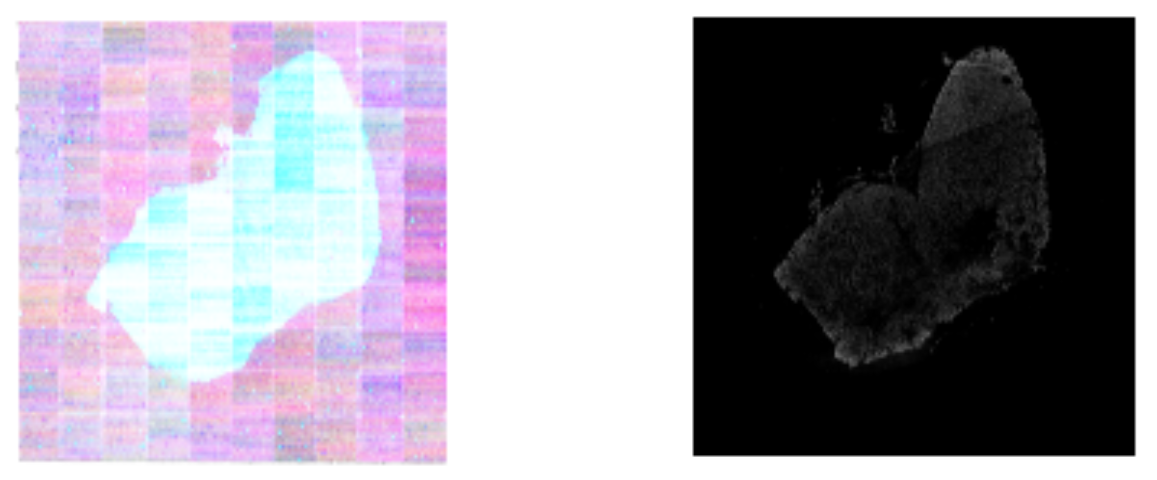
\includegraphics[scale=0.35]{../figures/imc_stpt_img4report.png}
	\caption{STPT (left) and IMC (right) images}		
\end{figure}

%-------------------------------------------------------------------------
\subsection{Image Preprocessing}

While training, we found that our hardware was not able to handle raw STPT and IMC images because of their large size. STPT images are (20800x20800) and IMC images are (18720x18720) while being both 16-bit images. Therefore, we resorted to crop each image into smaller chunks so that our network could train on these smaller images. 

First, we performed normalization and log scaling on all images. Next, for STPT images, we concatenated the two optical sections per physical section, giving 8-channeled tensors; for IMC images, we concatenated all 40 2D grayscale images per physical section, giving 40-channeled tensors. Since STPT images were slightly larger than IMC images, we resized each STPT image to (18720x18720) to match the size of IMC images. Finally, we used the function torch.split from the PyTorch library to crop original images into 256x256 chunks. See Figure 2 for an example of a chunk image. See Additional Details for more details on chunks. We treated this collection of 256x256 chunks as our new dataset. 

\begin{figure}[!h]
	\centering
	\captionsetup{justification=centering}
		\hspace*{-0.2cm}	
		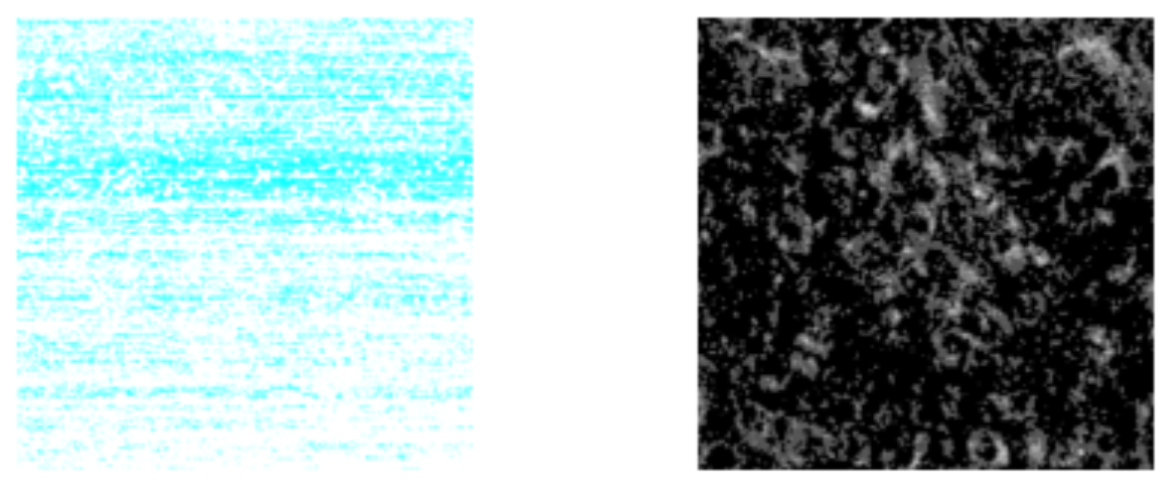
\includegraphics[scale=0.35]{../figures/sample_imc_stpt_crop.png}
	\caption{Cropped images from STPT (left) and IMC (right)}		
\end{figure}


%-------------------------------------------------------------------------
\subsection{U-Net}

We used the U-Net architecture \cite{ronneberger_2015_unet} as a benchmark to our point-cloud inspired architecture described in the next subsection. Our network architecture was nearly the same to that of the original U-Net paper. We only differed in including batch normalization layers after each ReLU application. We used mean-squared error (MSE) and the AdamW \cite{loshchilov_2017_decoupled} optimizer with learning rate 0.001 and weight decay 0.01 for training. 10\% of the images were randomly selected to make up the validation set. We also ensured that the validation set contained images from all physical sections. Minibatches of size 64 were used and the model was trained for 20 epochs.


%-------------------------------------------------------------------------
\subsection{PointSetGen}

3D data are becoming ubiquitous because of technological advancements in applications such as robotics, autonomous driving, and virtual reality \cite{wu_2020_pointconv}. Point clouds, a collection of (x,y,z) points in Euclidean space, are one of many representations of 3D data \cite{qi_2016_pointnet}. Special considerations must be taken into account when working with point clouds. For example, algorithms typically employ a symmetric function to respect the permutation invariance of point clouds. 

We trained the ‘hourglass’ neural network architecture from the PointSetGen paper by Fan et al. \cite{fan_2016_a}. The original aim in the paper was to reconstruct a 3D point cloud object from a single colored 2D image. In our application, we noted that IMC images of individual channels resembled point clouds and STPT images were essentially multi-channeled 2D images. Hence, the reconstruction task from STPT to IMC images was akin to the one described in Fan et al.
 
We followed the architecture described in Fan et al. ReLU activation functions and batch normalization were done after convolutional layers.  The output according to the original architecture in Fan et al. is an (Nx3) tensor, where N is the number of points in the final point cloud. However, since IMC images are not truly point clouds, but 2D grayscale images, we converted the (Nx3) tensor outputted by the original architecture to a 2D image using a custom point cloud rendering technique (See Additional Materials).

%------------------------------------------------------------------------
\section{Results}

To evaluate performance of the U-Net-based and the point cloud-based model, we selected a subset of cropped STPT images for reconstruction. Cropped STPT images were chosen based on how informative they were of the model’s performance from a visual standpoint. We ran forward passes on selected STPT images to obtain reconstructed IMC images. Each forward pass generated 40 2D grayscale images packaged in a 40-channel tensor – each channel corresponding to a different protein marker. For convenience, we only visualized reconstruction on 3 randomly chosen channels. We compared each model’s reconstructed IMC image by plotting both reconstructed and ground truth images using matplotlib, and by recording mean-squared error rounded to the second decimal place.


\subsection{U-Net}
Loss values for the U-Net model during training can be found in Figure 3. The loss is quite constant throughout training iterations, suggesting that the model is not learning. However, the loss curve does seem to exhibit a slight downward trend, but we do not believe the trend significant enough to make any conclusions. More training iterations are required to observe whether the downward trend continues. The shape of the loss curve could imply that the U-Net model was not able to pick up on the grain-like structures present in IMC images, since it was originally used in cell segmentation where cells were relatively large. 1

Figures 4-7 show reconstructed and ground truth images produced by our U-Net architecture. Each set of 3 reconstructions portray images of 3 randomly selected channels corresponding to a randomly chosen physical section and a selected chunk from the original image (see the Additional Materials for how to interpret chunks). Reconstructed images are on the left column and ground truth images are on the right column. Each row corresponds to a reconstructed / ground truth image pair. MSE values for each reconstruction pair (top, middle, bottom) is recorded in the captions of each figure.  

\begin{figure}
	\centering
	\captionsetup{justification=centering}
		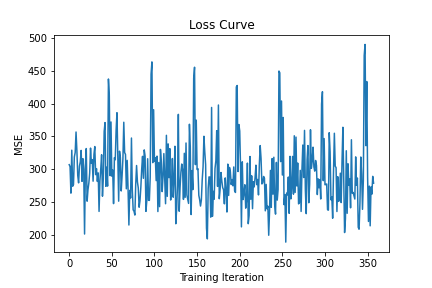
\includegraphics[scale=0.5]{../figures/unet_loss_curve.png}
	\caption{Loss curve for U-Net model. Mean squared error (MSE) in the y-axis and Training iteration on the x-axis}		
\end{figure}

%\clearpage
We observed poor reconstructions overall. The reconstructions did not seem to capture fine details present in ground truth images. The reconstructed image for physical section 12 chunk 30/41 in Figure 7 showed slightly better results than the reconstructed image for physical section 7 chunk 40/20 and physical section 3 chunk 40/20 in Figures 4 and 5 respectively. The network was able to accurately reconstruct the black background as seen in Figure 5.

\newpage 
\begin{figure}
	\centering
	\captionsetup{justification=centering}
		\hspace*{-0.8cm}	
		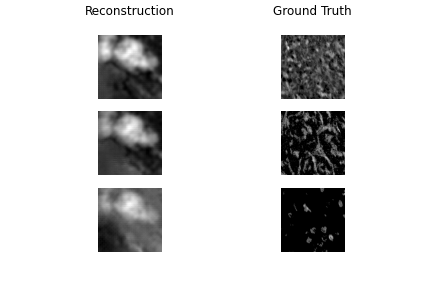
\includegraphics[scale=0.60]{../figures/7_40_20.png}
	\caption{Physical Section 7 chunk 40/20\\ MSE: 288.13 (top), 269.04 (middle), 274.63 (bottom)}		
\end{figure}


\begin{figure}
	\centering
	\captionsetup{justification=centering}
		\hspace*{-0.8cm}	
		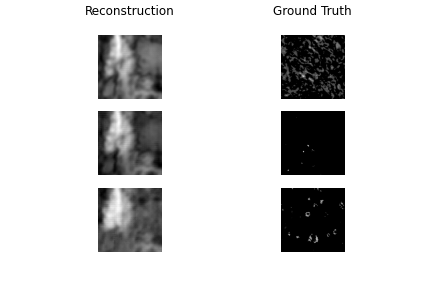
\includegraphics[scale=0.60]{../figures/3_40_20.png}
	\caption{Physical Section 3 chunk 40/20\\ MSE: 243.47 (top), 277.61 (middle), 272.33 (bottom)}		
\end{figure}


\begin{figure}
	\centering
	\captionsetup{justification=centering}
		\hspace*{-0.8cm}	
		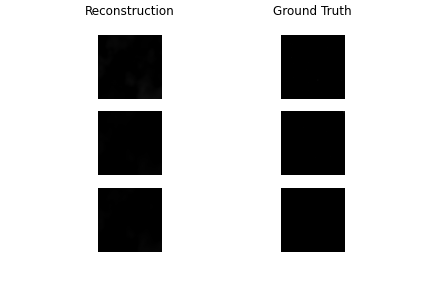
\includegraphics[scale=0.60]{../figures/10_40_35.png}
	\caption{Physical Section 3 chunk 40/35\\ MSE: 1.8 (top), 0.3 (middle), 0.2 (bottom)}		
\end{figure}


\begin{figure}
	\centering
	\captionsetup{justification=centering}
		\hspace*{-0.8cm}
		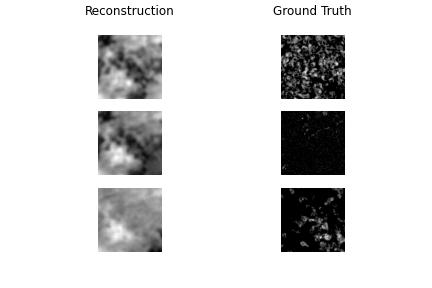
\includegraphics[scale=0.60]{../figures/12_30_41.png}
	\caption{Physical Section 12 chunk 30/41\\ MSE: 207.42 (top), 276.92 (middle), 264.55 (bottom)}		
\end{figure}

\newpage

\subsection{PointSetGen}
Our hardware resources prevented proper training of our PointSetGen architecture. Since the `hourglass' version of PointSetGen contains many convolutional layers, it was very memory demanding. We tried various workarounds to evade this problem. First, we lowered the batch size to 1, but still encountered the same memory issues. Next, we converted our model and images to 32-bit floats, which removed the memory issue, but produced nan loss values due to numeric instability. We could also fix the memory issue by using PyTorch's automatic mixed precision package torch.cuda.amp, which performs some operations using torch.float32 datatype and other operations using torch.float16, depending on numerical precision demands. 

We thought the numeric instability may come from model parameters going to inf, -inf or nan at some point during training. In an effort to combat numeric instability, we applied the He weight and bias initialization technique (He et al., 2015) when initializing the model parameters, which unfortunately did not resolve the problem. We also tried to lower the learning rate, but to no avail.


\section{Future Directions}
Our computing resources were very limited given the amount of time, so we were not able to train for many epochs in the case of the U-Net model. Therefore, in later iterations of the project, it would be advantageous to gain access to a cluster with more computing power. Greater computing power could further interrogate the slight downward trend described in Section 3.1.

In the case of our point cloud model, the numeric instability warrants additional time spent in debugging. Some other considerations that could improve performance include hyperparameter tuning, assessing different types of loss functions such as the binary cross entropy (BCE) loss, and exploring data augmentation methods such as elastic deformation.

\section{Conclusion}
In this study, we attempted to reconstruct IMC images from STPT images, which is useful in bio-medical imaging applications for mitigating costs and reducing inconsistencies during imaging. We constructed an image preprocessing pipeline to crop raw images to smaller (256x256) chunks to comply with GPU memory constraints for exploiting parallelization. 

We also implemented two separate neural network architectures to evaluate whether viewing IMC images as point clouds improved reconstruction performance. The first architecture was based on the well known U-Net architecture introduced by Ronneberger et al. \cite{ronneberger_2015_unet}. We observed poor reconstruction results from the U-Net architecture through qualitative and quantitative analysis. U-Net reconstructed images did not pick up the fine details of ground truth IMC images and had an average reconstruction error using MSE of about 270. Moreover, the loss curve seems to fluctuate around the same value, indicating the model is not learning effectively. 

The second network architecture was based on PointSetGen \cite{fan_2016_a}. This architecture was substantially larger compared to U-Net, so we encountered many memory problems during training. We tried to lower batch size, change the data types of tensors, and perform automatic mixed precision training using torch.cuda.amp. Although we were able to fix the memory issue, we could not resolve the numerical instability problems that arose as a result of our workarounds. This is an ongoing area of work for us.

It is still ambiguous at the moment how effective a neural network can be in reconstructing IMC images from STPT images. Moreover, it is unclear whether viewing IMC images as point clouds is indeed beneficial when constructing neural architectures. Further work must be done to verify this hypothesis.

\section{Code Availability}
Code is available at https://github.com/keviny2/stpt2imc/tree/main


\section{Additional Materials}
\subsection{Rendering Point Clouds as a 2D image}
First, we first constructed two 256x256 mesh grids using torch.meshgrid and concatenated them to a (2x256x256) tensor. Next, we extracted the x and y coordinates from the (Nx3) tensor, to form an (Nx2) tensor. We then used the gaussian equation to compute the intensity of each pixel, resulting in an (Nx256x256) tensor. This operation allowed gradients to flow through via coordinates to make training feasible. Refer to the Additional Materials for more details. We also constructed a separate multilayer-perceptron (MLP) that applies a convolutional layer to the last hidden layer of the neural network and outputs a (40xN) tensor. Finally, we perform element-wise multiplication between the tensor from the gaussian equation operation and the tensor from the MLP, ultimately giving us a (40x256x256) tensor; 40 2D images of size (256x256) for each protein marker. 


Generally speaking, let uv be a tensor with shape (HxWx2), xy be a tensor with shape (Nx2) and x be a tensor with shape (CxN). The following piece of code describes the gaussian equation to compute the intensity of each pixel. The result is a (40x256x256) image, provided the MLP outputs a 40-channeled tensor.

\begin{verbatim}
	torch.exp(((uv[None,:,:,0]
	            -xy[:,None,None,0])**2
	    + (uv[None,:,:,1]
	       -xy[:,None,None,1])**2)
	    / (xy[:,None,None,2]**2+1)) * MLP(x)
\end{verbatim}

\subsection{Chunks}
We form a grid on each STPT and IMC image when cropping original raw images. Each grid component is a (256x256) tensor. Therefore, (18720x18720) images will be sectioned into a (72x72) grid, each element in this (72x72) grid being a (256x256) cropped image (however, the last row and column are of size (32x32) because 18720 is not perfectly divisible by 256). We used 'chunk xx/yy' to locate where a specific cropped image lies in the original raw image. The 'xx' refers to the row index and 'yy' refers to the column index of the (72x72) grid. Therefore, 'chunk 30/41' would refer to the square whose top left corner's coordinates are (7424,10240) and bottom right coordinates are (7679, 10495) on the original raw STPT or IMC image.



%%%%%%%%% REFERENCES
{\small
\bibliographystyle{ieee_fullname}
\bibliography{my_bib}
}

\end{document}
